\documentclass[border=6pt]{standalone}
\usepackage{tikz}
\usetikzlibrary{arrows.meta,positioning,calc,shapes.geometric,fit,backgrounds,patterns,matrix,decorations.pathreplacing}
\begin{document}
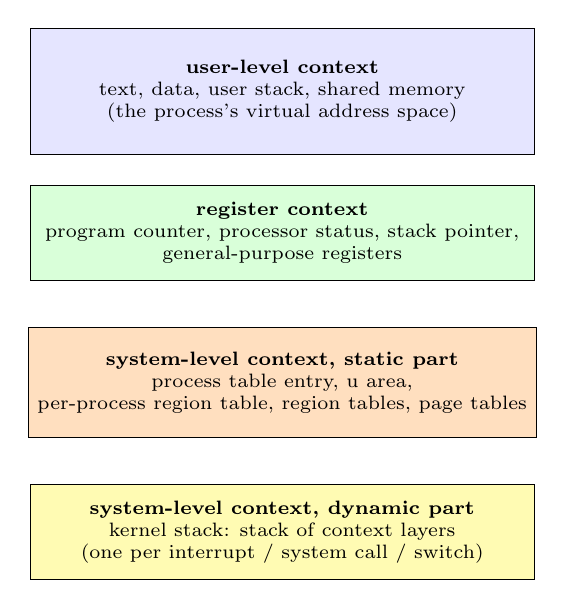
\begin{tikzpicture}[>=Stealth,font=\small]
\tikzstyle{b}=[draw,minimum height=0.6cm,minimum width=6.4cm,font=\scriptsize,align=center]
\node[b,fill=blue!10,minimum height=1.6cm] (u) at (0,2.0) {\textbf{user-level context}\\ text, data, user stack, shared memory\\ (the process's virtual address space)};
\node[b,fill=green!15,minimum height=1.2cm] (r) at (0,0.2) {\textbf{register context}\\ program counter, processor status, stack pointer,\\ general-purpose registers};
\node[b,fill=orange!25,minimum height=1.4cm] (s) at (0,-1.7) {\textbf{system-level context, static part}\\ process table entry, u area,\\ per-process region table, region tables, page tables};
\node[b,fill=yellow!30,minimum height=1.2cm] (d) at (0,-3.6) {\textbf{system-level context, dynamic part}\\ kernel stack: stack of context layers\\ (one per interrupt / system call / switch)};
\end{tikzpicture}
\end{document}
